% Chapter Template

\chapter{Introduction} % Main chapter title

\label{ch:introduction} % Change X to a consecutive number; for referencing this chapter elsewhere, use \ref{ChapterX}

Surface normal is an important property of a surface with many applications, like surface reconstruction, shadings generation and other visual effects. However, the calculation of surface normal in many tasks is not as straightforward as simply the cross-product of two plane vectors. Especially in the task of real-world object digitalization, the surface is usually hardly to be mathematically described in equations due to the elaborate details on the objects. Instead, it is common to use a group of points to describe the object surface, which is a memory economical solution to save the fine detail of the objects and also can be easier measured by 3D scanners. Therefore the task is converted to the normal inference based on the surface point, and the most of the case, the result surface normal is merely an approximation. 

\begin{figure}[h!]
	\centering
	{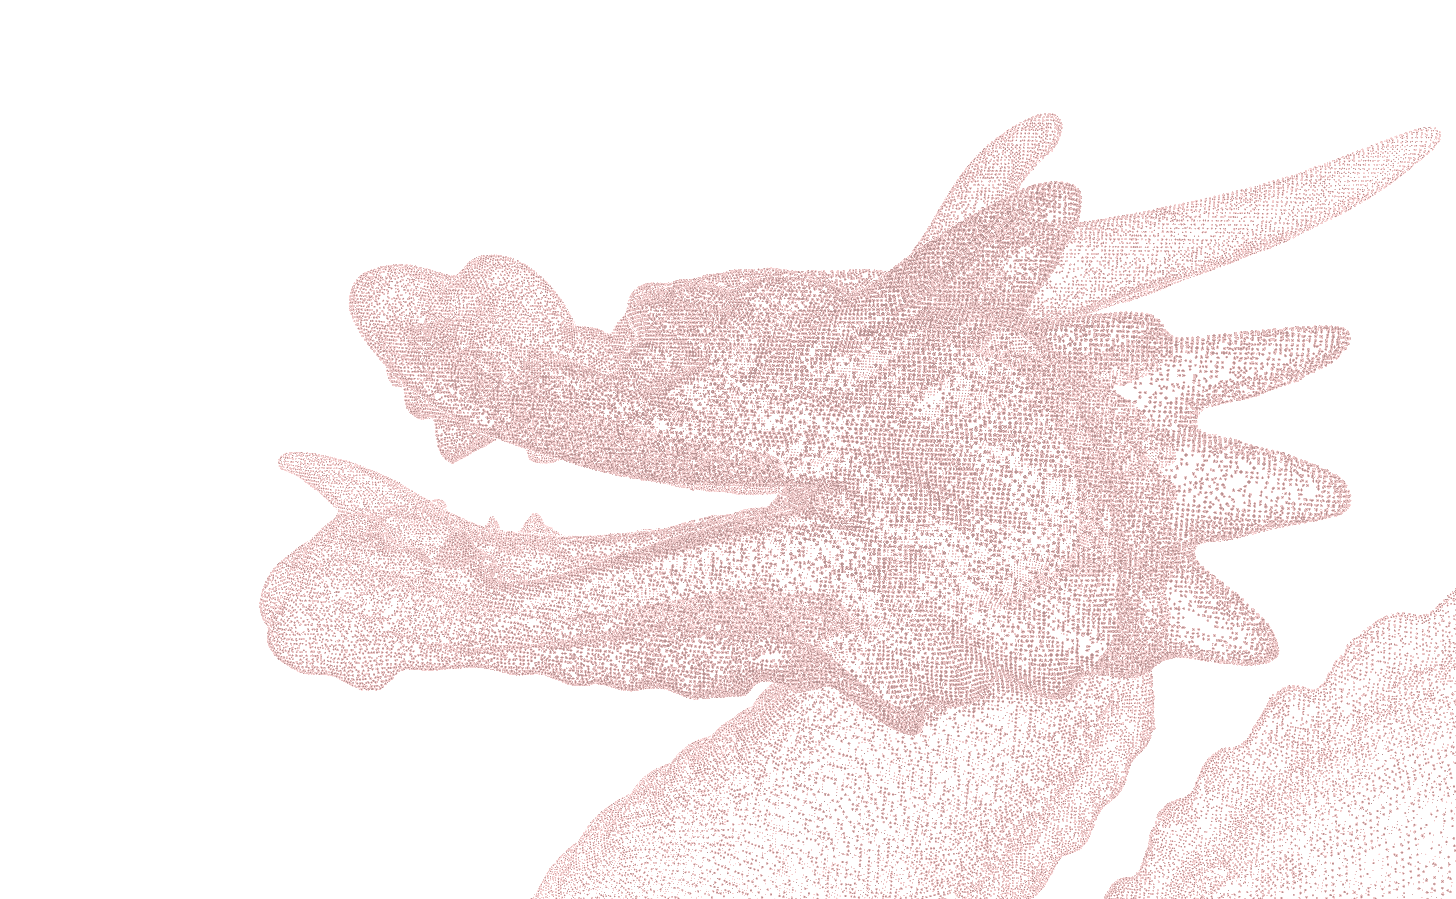
\includegraphics[width=.45\textwidth]{./Figures/point-cloud.png}};
	{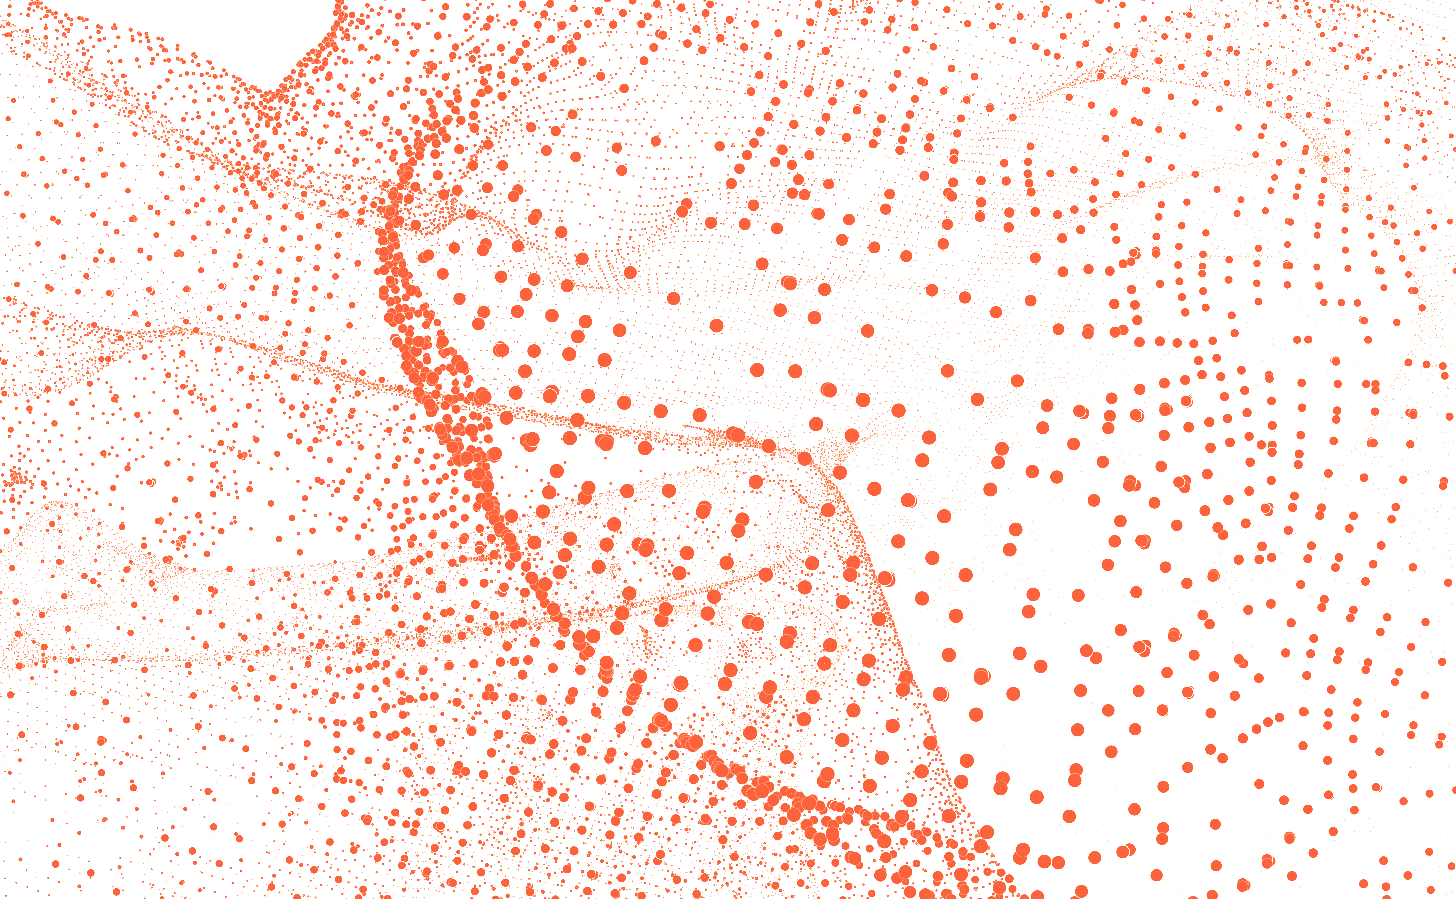
\includegraphics[width=.45\textwidth]{./Figures/point-cloud-zoom-in.png}};
	\decoRule
	\caption{Left: A part of the point cloud of the dragon model. Right: The zoom in of the left point cloud.}
	\label{fig:point-cloud}
\end{figure}

Apart from this, due to the application scenarios, the working principle of scanners are various, which consequently produce point cloud structures in different forms. For the scanners without positions recording, the point cloud acquired after scanning is unstructured. In this case, every 3D point can be captured by different capture position, and neighbors are not defined by capture time. It increases the difficulty and computation for the neighbor based normal inference approaches.  Furthermore, since the lack of inherent structure, the normal can hardly be inferred by the parallel approaches. 

However, for the scanner with calibrated camera, a structured point cloud can be captured. One example is the depth camera. It captures the RGB-D images for the object, which includes the standard RGB image with depth information of each pixel. After camera calibration, a corresponding point cloud can be calculated based on the depth map and camera matrix. It gives the advantage that a structured point cloud is mapped directly based on the same capture position from a 2D depth map, the neighbor information of each point is identical to the corresponding pixel in the 2D depth map. It provides a better view for the normal inference task since the neighbor information can be considered as an important reference.
Besides the point cloud, which is one piece of information can be used for normal reference, the RGB image also leaves the trace of surface normal. If assume object surface is diffuse and the light coming from a knowing direction , the brightness of the object surface is proportional to the surface normal, which is known as Lambertian surface. It indicates the normal inference task can also utilize the relationship between surface normal and light reflection to further rectify the inferred normal map with knowing light source. Therefore, the illuminated calibrated RGB-D image provides as a good input for normal inference tasks.
Unfortunately, in the actual situation, the depth maps captured by the sensors are only semi-dense, which is mainly caused by optical noises and the reflections in dark and shinny areas. Consequently, it disrupts the robustness of the normal inference methods. Median filters can be used for the sparse missing pixels, however, for the case of huge missing holes in the depth map, it produces just a paltry result. Thus a reasonable guess is required for missing areas.

Deep learning based methods provides multiple possible solutions for the challenges mentioned above. First, to deal with the noised input, deep learning based methods already have the solution for the similar tasks like image inpainting and depth density enhancement, which base on the noised image as input to predict the clean and fully dense output with or without original meanings. Therefore, it can be a help for noise in the depth map. Besides, the network of deep learning model can also handle the structured point cloud as a single input and infer the corresponding normal all together, which is very time economical comparing to the approaches like neighbor based methods. In addition, the multi-stages training architectures provide a way to consider both depth map and texture image as the input to predict the surface normals, which not only consider the point cloud but also the add the lambertian reflection as a further constraint.

In this work, we focus on the normal inference based on a semi-dense depth map with RGB image using deep learning based approaches. Specifically, the missing pixels in the depth map is filled up by the gated convolution and propagate in a customized UNet with skipping connections. The output of the training model is directly the surface normal corresponding the input depth map. The grayscale image is used to further improve the estimation accuracy. 
For the training work, a dataset named “synthetic50-5” is created including 55 high resolution point clouds from internet, as shown in Appendix A. The point clouds provide with the high accurate normals, which can be used as the ground truth of the training work. Most of the models have elaborate details with high curvatures but also contain smooth surfaces. The trained model is evaluated on both synthetic dataset as well as the real dataset captured from RGB-D cameras. A series of metrics have been used for qualitative evaluation. The model is shown to achieve a remarkably better prediction accuracy at a low computational cost compared to the standard approaches for semi-dense point clouds.  

The structure of the thesis is as follows, Chapter 1 is the introduction of the whole work. Chapter 2 briefly discusses the related work about normal inference. Chapter 3 is the main approaches of this work. Chapter 4 introduces the created dataset for the training work. Chapter 5 is the description of the experiments and the evaluation of the models. Chapter 6 is the conclusion of the whole thesis.



